This section describes the interaction of particles with matter, focusing on the particles and energy range relevant for this thesis, electrons ($0-18~\keV$) and photons in the visible range (approx. $380-750~\nm$).

Electrons have charge so their interaction with matter is mainly with the orbital atomic  electrons through the Coulomb force. The electron trajectory is much more tortuous than other heavier particles because the mass of both interacting particles is equal. Furthermore, for the same reason, these electrons lose a significant amount of energy in each collision. The specific energy loss is defined as $S=-\frac{dE}{dx}$ which gives the energy loss suffered by the particle per unit of path length. In the case of electrons, this total energy loss has two main contributions, the collisions (elastic and inelastic) and radiative processes (bremsstrahlung) \cite{Knoll, Leo}:

\begin{equation}
\frac{dE}{dx} \approx \left(\frac{dE}{dx}\right)_{c} + \left(\frac{dE}{dx}\right)_{br} 
\label{eq:ElectronInteraction}
\end{equation}

The radiative part is roughly proportional to the collision part:
\begin{equation}
\frac{\displaystyle{\left(\frac{dE}{dx}\right)_{br}}}{\displaystyle{\left(\frac{dE}{dx}\right)_{c}}} \approx \frac{EZ}{700}
\label{eq:ProportionalMagnituds}
\end{equation}
where $E$ is the energy of the electron in $\MeV$ and $Z$ is the atomic number of the absorbing material. Due to this energy loss, the electrons can only penetrate a material as far as they go before losing their total kinetic energy. This distance is known as range and, in the case of tritium electrons, its value is quoted in Table \ref{tab:MeanFreePathTritium}.

As photons don't have charge, their possible interactions with the matter are photoelectric effect, Compton effect, coherent scattering and pair production and the probability of each process depends on the energy of the photon, $E_\gamma = h\nu$, and on the atomic number of the material, Z, displayed in Figure \ref{fig:ProcessesPhotons}.

\begin{figure}[h]
\centering
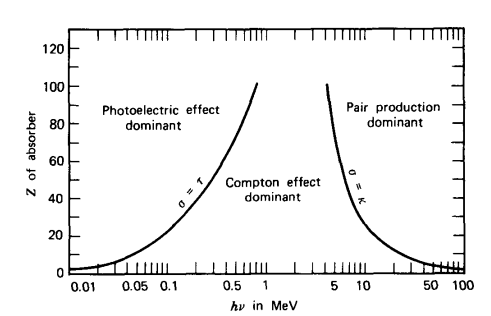
\includegraphics[scale=0.75]{3DesignPrinciples/32Tritium_detector/DominantProcessesPhotons.png}
\caption{Domain regions of the three most probable types of interactions of gamma rays with matter. The lines show the values of Z and $h\nu$ where the two neighboring effects are equally likely.\label{fig:ProcessesPhotons}~\cite{Knoll, Leo}}
\end{figure}

The only relevant photons for this thesis are in the visible range, between $400$ and $700~\nano\meter$, that corresponds to energies of the order of the $\eV$. Therefore, pair productions, which requires a photon energy equal or more than $1.022~\MeV$, does not play any role.

The photoelectric effect occurs when a photon interacts with an orbital electron in the material, losing all its energy. This energy is absorbed by the electron that is released from the atom (ionization). The energy of the resulting electron, $E_e$, is \cite{Knoll, Leo}:
\begin{equation}
E_e = E_\gamma - E_b 
\label{eq:PhotoelectricEffect}
\end{equation}
where $E_b$ is the binding energy of the electron in this material. The probability of this effect depends on the number of available electrons in the matter through the variable Z, and the energy of the electron according to the expression \cite{Knoll}:

\begin{equation}
\left(Pr\right)_{Ph-eff} \approx \frac{Z^n}{E_\gamma^{3.5}}
\label{eq:PhotoelectricProb}
\end{equation}

Thus, the photoelectric effect is most probable for elements with high atomic number. This is the reason why elements with high atomic number are the best isulators against gamma radiation and why the passive shielding of TRITIUM monitor consists of lead bricks ($Z=82$) (section \ref{subsec:SetUpPassiveShield}). %This is also the reason why elements with high atomic number like $\ce{Sb}$ ($Z=51$), $\ce{Rb}$ ($Z=37$) or $\ce{Cs}$ ($Z=55$), are used in the cathodes of PMTs. 

The Compton effect occurs when a photon interacts with an orbital electron of the material, transferring part of its energy to the electron, which is released, scattered at an angle $\theta$ with respect to the original direction. If the electron binding energy is neglected, the energy transfered to it, $E_e$, is given by \cite{Knoll, Leo}:
\begin{equation}
E_e=\frac{\frac{E_\gamma^2}{m_oc^2}\left(1-cos\theta\right)}{1+ \frac{E_\gamma^2}{m_oc^2}\left(1-cos\theta\right)}
\label{eq:ComptonEffect}
\end{equation}
where $m_0$ is the rest mass of the electron and $c$ is the speed of the light in the vacumm. The probability of the Compton effect is proportional to the atomic number (available electrons in the matter), Z,  and decreases with the energy of the photon. 

As can be seen in Figure \ref{fig:ProcessesPhotons}, for photon energies in the visible spectrum (of the order of eV), the Compton effect is only likely for very light materials, (Z<4). For heavier materials the photoelectric effect is the dominant effect.

Finally, for coherent scattering, the atom is neither excited nor ionized and the photon conserve all its energy in the collision. Coherent scattering is more probable for photons with low energies and materials with high atomic numbers and, as it will be shown in section \ref{subsec:PlasticScintillators}, it explains why the produced photons are guided along scintillating fibers. 


%Because of the fact that the energy of the photon doesn't change we will not speak more about this effect but it is important since this effect change de direction of photons and it will affect to their mean free path.